
\documentclass[../relatorio.tex]{subfiles}
\begin{document}
De forma a ilustrar alguns dos diagramas de sequência desenvolvidos, foram escolhidos 3 use cases com o objetivo de 
apresentar todos os diagramas referentes a estes e também qual foi a estratégia escolhida para os resolver.
Foram considerados 3 \textit{uses cases} "principais", nomeadamente o Fazer Orçamento, o Realizar Reparação e ainda o
Pedir reparação expresso.

\subsection{Fazer Orçamento}
Tal como é referido no use case, quando o técnico pretende fazer um orçamento, este solicita o pedido de orçamento mais 
antigo. O sistema para responder a este pedido, constroi um Set ordenado por ordem descrescente da data de criação com todos os Orçamentos 
em que o estado é "porCalcular". Set este construído a partir do método getOrcamentosAtivos(), chamado pelo getOrcamentoMaisAntigo() que lhe retira
o primeiro elemento.
\begin{figure}[!ht]
    \centering
    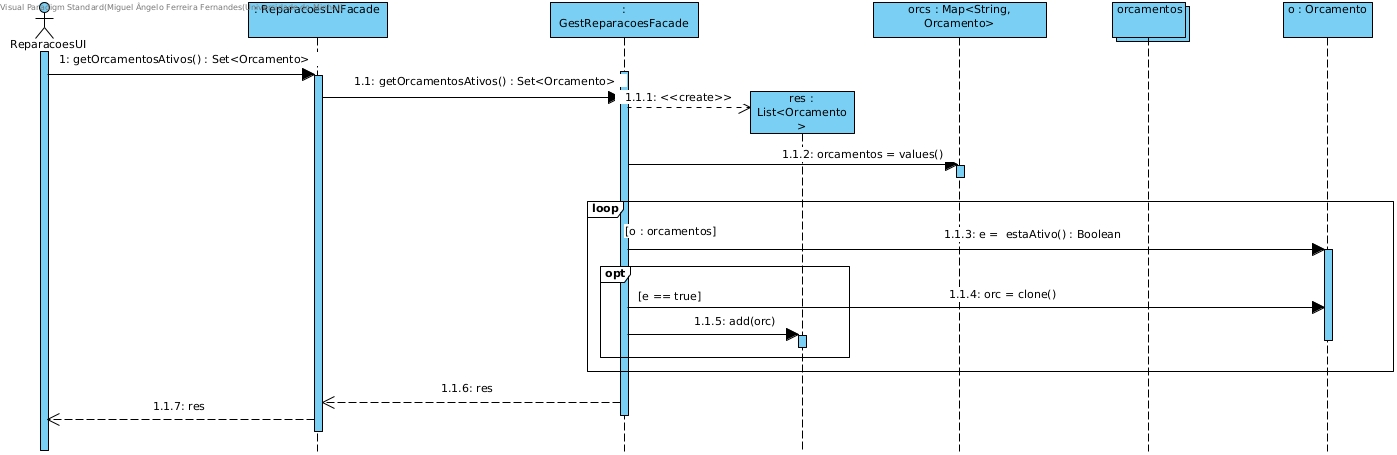
\includegraphics[scale=0.45]{../assets/diagramas_sequencia/sd-GetOrcamentosAtivos.jpg}
    \caption{Diagrama de \textit{Use Case}}
\end{figure}

Depois de saber qual o Orçamento que tem de calcular, o técnico analisa o equipamento e vai construindo o plano de trabalhos adicionando 
sequencialmente os passos necessários para a sua reparação. Cada passo é identificado por um nome e é caracterizado pelo tempo estimado e ainda
por o material que é expectável usar.

\begin{figure}[!ht]
    \centering
    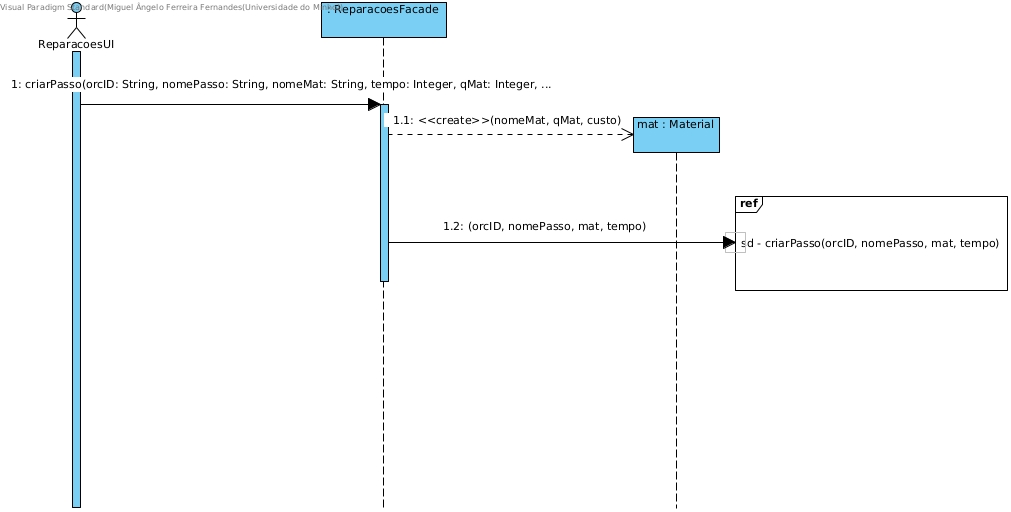
\includegraphics[scale=0.45]{../assets/diagramas_sequencia/sd-criarPasso1.jpg}
    \caption{Diagrama de \textit{Use Case}}
\end{figure}

\begin{figure}[!ht]
    \centering
    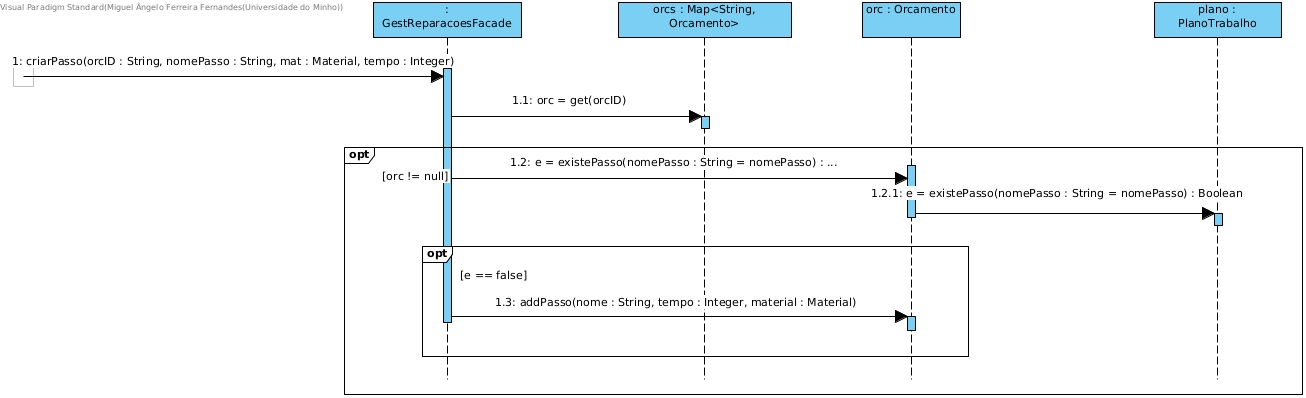
\includegraphics[scale=0.45]{../assets/diagramas_sequencia/sd-criarPasso2.jpg}
    \caption{Diagrama de \textit{Use Case}}
\end{figure}

Quando todos os passos já foram adicionados e o plano de trabalhos já foi concluído o técnico pode gerar o Orçamento e registar o 
envio do mesmo ao cliente. O estado do orçamento muda de "porCalcular" para enviado e é adicionado às comunicações do Orçamento o 
contacto referente ao envio.

\begin{figure}[!ht]
    \centering
    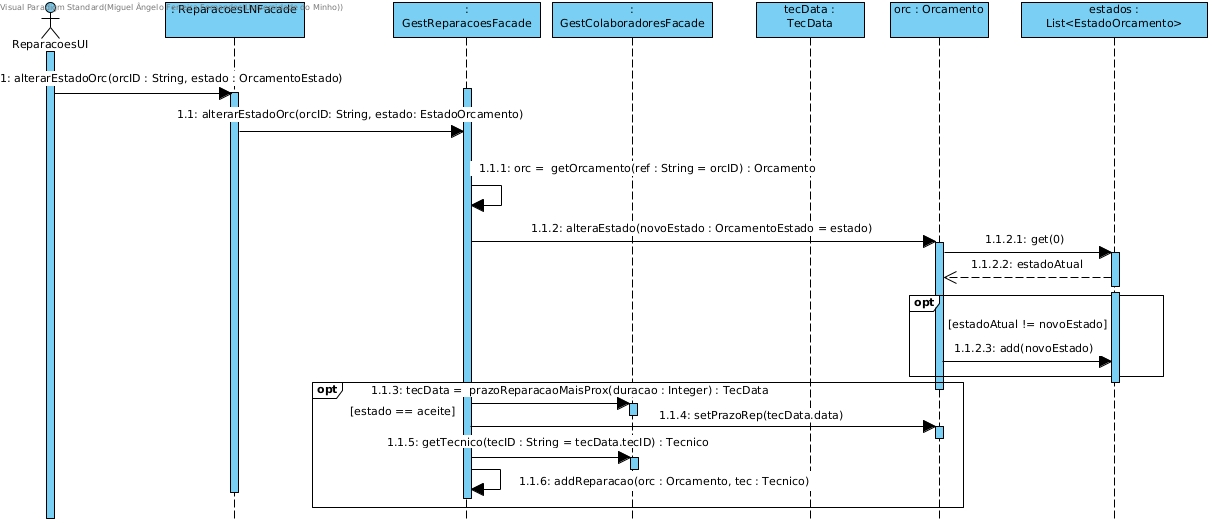
\includegraphics[scale=0.45]{../assets/diagramas_sequencia/sd-alterarEstadoOrc.jpg}
    \caption{Diagrama de \textit{Use Case}}
\end{figure}

\begin{figure}[!ht]
    \centering
    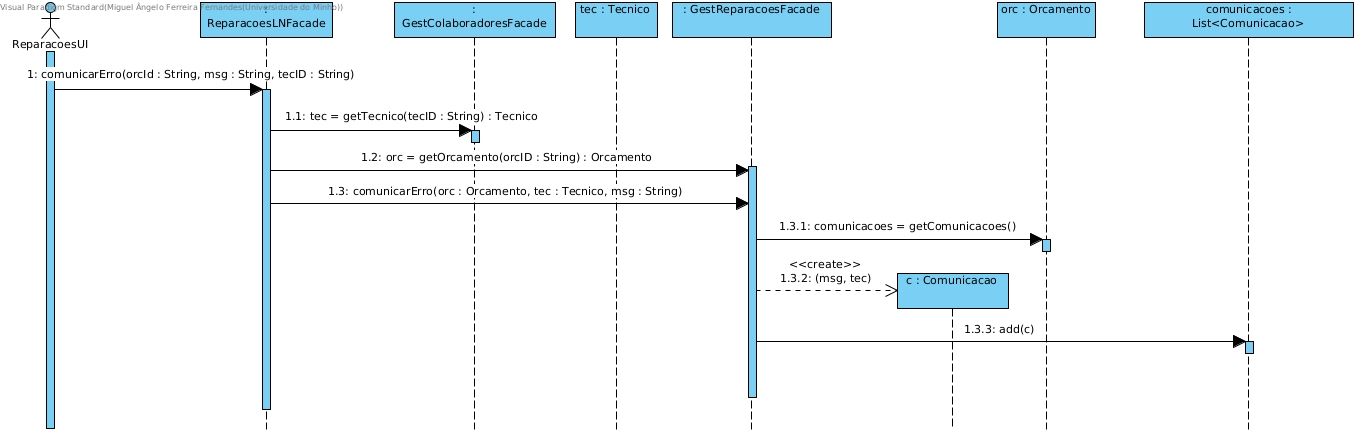
\includegraphics[scale=0.45]{../assets/diagramas_sequencia/sd-ComunicarErro.jpg}
    \caption{Diagrama de \textit{Use Case}}
\end{figure}
    
\end{document}